\subsection{SatImgNet}
{{\footnotesize
\noindent SATIN (sometimes referred to as SatImgNet) is a multi-task metadataset of 27 satellite
imagery classification datasets evaluating zero-shot transfer of vision-language models
across diverse remote sensing tasks.


\begin{description}[labelwidth=4cm, labelsep=1em, leftmargin=4cm, itemsep=0.1em, parsep=0em]
  \item[date:] 2023-04-23
  \item[version:] 1
  \item[last\_updated:] 2023-04-23
  \item[expired:] false
  \item[valid:] yes
  \item[valid\_date:] 2023-04-23
  \item[url:] \href{https://huggingface.co/datasets/saral-ai/satimagnet}{https://huggingface.co/datasets/saral-ai/satimagnet}
  \item[doi:] 10.48550/arXiv.2304.11619
  \item[domain:] Remote Sensing
  \item[focus:] Satellite imagery classification
  \item[keywords:]
    - land-use
    - zero-shot
    - multi-task
  \item[licensing:] CC-BY-4.0
  \item[task\_types:]
    - Image classification
  \item[ai\_capability\_measured:]
    - Zero-shot land-use classification
  \item[metrics:]
    - Accuracy
  \item[models:]
    - CLIP
    - BLIP
    - ALBEF
  \item[ml\_motif:]
    - Transfer Learning
  \item[type:] Benchmark
  \item[ml\_task:]
    - Supervised Learning
  \item[solutions:] Numerous, evaluated via leaderboard
  \item[notes:] Public leaderboard available
  \item[contact.name:] Jonathan Roberts
  \item[contact.email:] j.roberts@cs.ox.ac.uk
  \item[datasets.links.name:] SatImgNet on Hugging Face
  \item[datasets.links.url:] \href{https://huggingface.co/datasets/saral-ai/satimagnet}{https://huggingface.co/datasets/saral-ai/satimagnet}
  \item[results.links.name:] SatImgNet Leaderboard
  \item[results.links.url:] \href{https://huggingface.co/spaces/saral-ai/satin-leaderboard}{https://huggingface.co/spaces/saral-ai/satin-leaderboard}
  \item[fair.reproducible:] True
  \item[fair.benchmark\_ready:] True
  \item[id:] satimgnet
  \item[Citations:] \cite{roberts2023satin}
\end{description}

{\bf Ratings:} ~ \\

\begin{tabular}{p{0.15\textwidth} p{0.07\textwidth} p{0.7\textwidth}}
\hline
Rating & Value & Reason \\
\hline
dataset & 5 & Hosted on Hugging Face, versioned, FAIR-compliant with rich metadata; covers many well-known remote sensing datasets unified under one metadataset, though documentation depth varies slightly across tasks.
 \\
documentation & 5 & Paper provides all required information
 \\
metrics & 5 & Accuracy of classification is an appropriate metric
 \\
reference\_solution & 4 & Baselines like CLIP, BLIP, ALBEF evaluated in the paper; no constraints specified
 \\
software & 0 & No scripts or environment information provided
 \\
specification & 4 & Tasks (image classification across 27 satellite datasets) are clearly defined with multi-task and zero-shot framing; input/output structure is mostly standard but some task-specific nuances require interpretation.
 \\
\hline
\end{tabular}

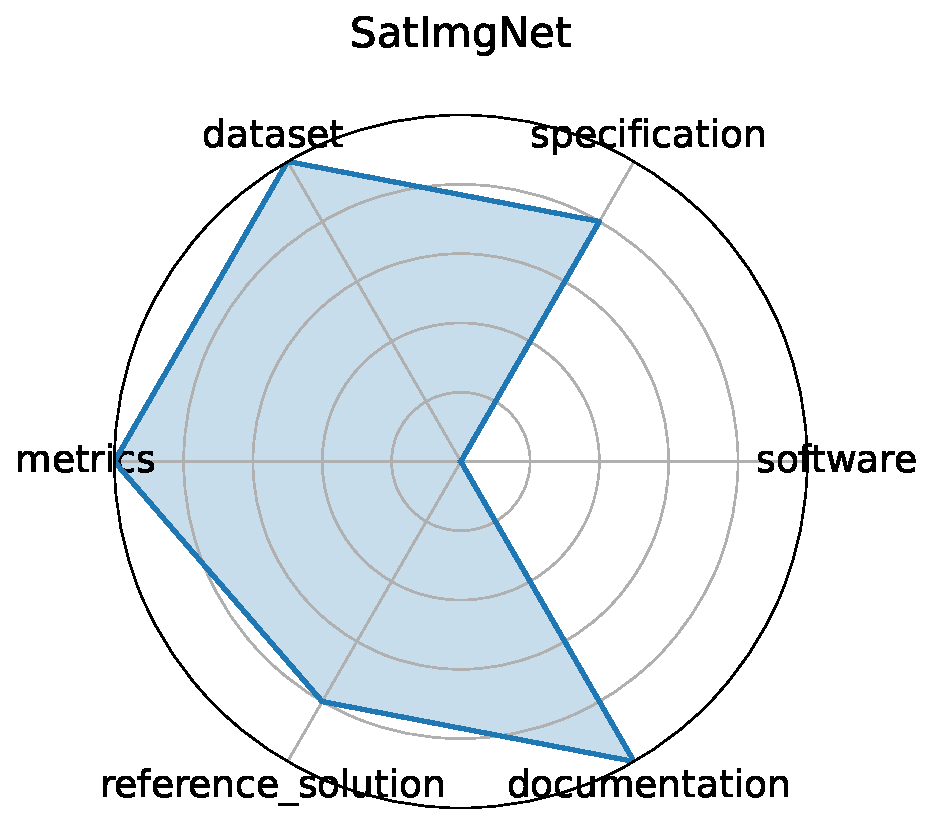
\includegraphics[width=0.2\textwidth]{satimgnet_radar.pdf}
}}
\clearpage